\documentclass[tikz, border=10pt]{standalone}
\usepackage{iftex}
\ifluatex
  \usepackage{fontspec}
  \usepackage{unicode-math}
  \setmainfont{Fira Sans}
  \setmonofont{Fira Mono}
  \setmathfont{Fira Math}
\else
  \usepackage[T1]{fontenc}
\fi

\usetikzlibrary{arrows.meta, calc}
\tikzset{every node/.style={font=\Large}}


\begin{document}
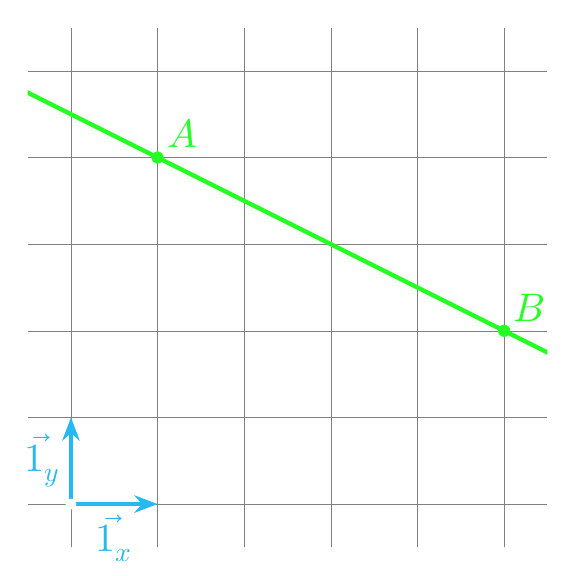
\begin{tikzpicture}[scale=1.1, >=Stealth]
  % Bounding box fixe (taille originale)
  \path[use as bounding box] (-0.5,-0.5) rectangle (5.5,5.5);

  % Colors tuned for dark preview background.
  \colorlet{axiscol}{white}
  \colorlet{gridcol}{white!50!black}
  \colorlet{datacol}{green!85!white}
  \colorlet{vecbasiscol}{cyan!85!white}

  % Cartesian grid.
  \draw[step=1, very thin, gridcol] (-0.5,-0.5) grid (5.5,5.5);

  % Basis vectors.
  \draw[->, very thick, vecbasiscol] (0,0) -- (1,0)
    node[midway, below, text=vecbasiscol] {$\vec{1_x}$};
  \draw[->, very thick, vecbasiscol] (0,0) -- (0,1)
    node[midway, left, text=vecbasiscol] {$\vec{1_y}$};

  % Points.
  \coordinate (A) at (1,4);
  \coordinate (B) at (5,2);
  \coordinate (O) at (0,0);

  % Points and labels.
  \fill[axiscol] (O) circle (1.8pt);
  \fill[datacol] (A) circle (2pt);
  \fill[datacol] (B) circle (2pt);

  \node[below left, text=axiscol] at (O) {$O$};
  \node[above right, text=datacol] at (A) {$A$};
  \node[above right, text=datacol] at (B) {$B$};

  % Droite AB "infinie" mais coupée dans le cadre
  \begin{scope}
    \clip (-0.5,-0.5) rectangle (5.5,5.5);
    \draw[ultra thick, datacol] ($(A)!-10!(B)$) -- ($(A)!10!(B)$);
  \end{scope}
\end{tikzpicture}
\end{document}
